\documentclass{amsart}
\usepackage{tikz}
\usetikzlibrary{arrows.meta}
\begin{document}
\section{Drafts}
\subsection{Equal length paths on a Manhattan grid}
\begin{figure}
  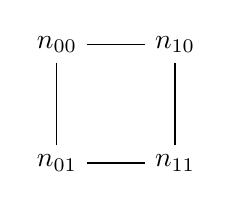
\begin{tikzpicture}[node distance={1.5cm}]
    \node (00) {$n_{00}$};
    \node (10) [right of=00] {$n_{10}$};
    \node (01) [below of=00] {$n_{01}$};
    \node (11) [right of=01] {$n_{11}$};

    \draw (00) edge (10);
    \draw (00) edge (01);
    \draw (10) edge (11);
    \draw (00) edge (10);
    \draw (01) edge (11);
  \end{tikzpicture}
\end{figure}

\end{document}